\documentclass{article}
% For math environments
\usepackage{amsmath, amsfonts}
% For links
\usepackage[hidelinks]{hyperref}
% So space it put between paragraphs
\usepackage{parskip}
% For figures
\usepackage{tikz}
% Set the margins to not be ridiculous
\usepackage[margin=0.75in]{geometry}
% For multiple columns
\usepackage{multicol}
% For controlling enum/itemize spacing and indentation
\usepackage{enumitem}

% For tikz plots
\usepackage{pgfplots}
% This isn't needed but avoids a compiler warning
\pgfplotsset{compat=1.16}

% Allow multi-line equations to be broken across pages
\allowdisplaybreaks

% Use @ as a letter
\makeatletter

% Scale down all tikz coordinates while maintaining font size
\tikzset{every picture/.style={scale=0.45, every picture/.style={}}}


% Macros
% Monospace code
\def\code#1{\texttt{#1}}

% Greek letters
\def\a{\alpha}
\def\b{\beta}
\def\g{\gamma}
\def\d{\delta}
\def\D{\Delta}

% Some common sets
\def\es{\varnothing}
\def\ints{{\mathbb{Z}}}

% Commands that make life easier
\newcommand\gath[1]{\begin{gather} #1 \end{gather}}
\newcommand\gaths[1]{\begin{gather*} #1 \end{gather*}}
\newcommand\ali[1]{\begin{align} #1 \end{align}}
\newcommand\parens[1]{\left( #1 \right)}
\newcommand\squares[1]{\left[ #1 \right]}
\newcommand\braces[1]{\left\{ #1 \right\}}
\newcommand\angles[1]{\left\langle #1 \right\rangle}
\newcommand\deriv[2]{\frac{d #1}{d #2}}
\newcommand\abs[1]{\left| #1 \right|}
\newcommand\floor[1]{\left\lfloor #1 \right\rfloor}
\newcommand\ceil[1]{\left\lceil #1 \right\rceil}
\DeclareMathOperator{\lcm}{lcm}
\def\non{\nonumber \\}
\newcommand\unit[1]{~\mathrm{#1}}
\newcommand\combos[2]{{}_{#1}C_{#2}}

% Set stuff
\def\ss{\subseteq}

% Multiline equation space
\def\mlesp{\hspace{1.2cm}}

% For grid diagrams
\newcommand\gridbox[3]{\draw (#1,#2) rectangle (#1+1,#2+1) node[pos=.5] {#3};}
\newcommand\gridboxh[3]{\draw[fill=red!20] (#1,#2) rectangle (#1+1,#2+1) node[pos=.5] {#3};}
\newcommand\gridboxb[3]{\draw[fill=black] (#1,#2) rectangle (#1+1,#2+1) node[pos=.5] {#3};}
\newcommand\gridsym[3]{\node at (#1+0.5,#2+0.5) {$#3$};}
\newcommand\gridblank[2]{\filldraw[draw=gray, color=gray] (#1,#2) rectangle (#1+1,#2+1);}
\newcommand\gridcirc[2]{\draw (#1 + 0.5,#2 + 0.5) circle (0.25);}
\newcommand\cwlab[3]{
  \def\dd{0.15}
  \draw (#1 + \dd - 0.03, #2 + 1 - \dd) node {\scriptsize #3};
}

\def\bbw{3.5}
\def\bbh{2}
\newcommand\bigbox[3]{\draw (#1*\bbw,#2*\bbh) rectangle (#1*\bbw+\bbw,#2*\bbh+\bbh) node[pos=.5] {#3};}
\newcommand\bbtextr[3]{\node[right] at (#1*\bbw,#2*\bbh+0.5*\bbh) {#3};}
\newcommand\bbtextb[3]{\node[align=center] at (#1*\bbw+0.5*\bbw,#2*\bbh+0.5*\bbh) {#3};}

% Box puzzle stock answer
\newcommand\boxans[1]{
  Logic was used to deduce the solution:

  #1

  This was verified using Python as well as shown to be unique with a brute force approach.
}

% Standard crossnumber grid
\newcommand\crossnumstd[9]{
  \begin{center}
    \begin{tikzpicture}[scale=2]
      \gridbox{0}{2}{#1}
      \gridbox{1}{2}{#2}
      \gridbox{2}{2}{#3}
      \gridbox{0}{1}{#4}
      \gridbox{1}{1}{#5}
      \gridbox{2}{1}{#6}
      \gridbox{0}{0}{#7}
      \gridbox{1}{0}{#8}
      \gridbox{2}{0}{#9}

      % Labels
      \cwlab{0}{2}{1}
      \cwlab{1}{2}{2}
      \cwlab{2}{2}{3}
      \cwlab{0}{1}{4}
      \cwlab{0}{0}{5}
    \end{tikzpicture}
  \end{center}
}

% Multiple numbers
\newcommand\mn[1]{$#1$'s}

% Commands for problems
\newcommand\problem[4]{
\section*{#1}

\textbf{Question:} #3

\textbf{Answer:} #2

\textbf{Explanation:} #4
}
\newcommand\aproblem[4]{\problem{Dec #1}{#2}{#3}{#4}}
\newcommand\cproblem[4]{\problem{Problem #1}{#2}{#3}{#4}}

\newcommand\xref@advent[2]{#1 Advent, Dec~#2 problem}
\newcommand\xref@card[2]{#1 Christmas Card, Problem #2}

% For answered verified with Python
\newcommand{\verified}{This was verified with a brute-force Python program.}

\def\advent@xxi@i{
  The geometric mean of a set of $n$ numbers can be computed by multiplying together all the numbers then computing the $n$th root of the result.

  The factors of $4$ are $1$, $2$ and $4$. The geometric mean of these is 2.

  The factors of $6$ are $1$, $2$, $3$, and $6$. The geometric mean of these is $\sqrt{6}$.

  The geometric mean of all the factors of today's number is $22$.
}

\def\advent@xxi@ii{
  The number $7n$ has $37$ factors (including $1$ and the number itself).
  How many factors does $8n$ have?
}

\def\advent@xxi@iii{
  If you write out the numbers from $1$ to $1000$ (inclusive), how many times will you write the digit $0$?
}

\def\advent@xxi@iv{
  Put the digits $1$ to $9$ (using each digit exactly once) in the boxes so that the sums are correct.
  The sums should be read left to right and top to bottom ignoring the usual order of operations.
  For example, $4 + 3 \times 2$ is $14$, not $10$.
  Today's number is the product of the numbers in the red boxes.

  \grid@advent@xxi@iv{}{}{}{}{}{}{}{}{}
}

\def\advent@xxi@v{
  How many different isosceles triangles are there whose perimeter is $50$ units, and whose area is an integer number of units squared?

  (Two triangles that are rotations, reflections and translations of each other are counted as the same triangle. Triangles with an area of 0 should not be counted.)
}

\def\advent@xxi@vi{
  When $12345$ is divided by today's number, the remainder is $205$.
  When $6789$ is divided by today's number, the remainder is $112$.
}

\newcommand\dec@ai{0.30901699437494745}
\newcommand\dec@aii{0.8090169943749475}
\newcommand\dec@bi{0.5877852522924731}
\newcommand\dec@bii{0.9510565162951535}
\newcommand\decagon[5]{
  \def\ai{\dec@ai*#3+#1}
  \def\aii{\dec@aii*#3+#1}
  \def\bi{\dec@bi*#3+#2}
  \def\bii{\dec@bii*#3+#2}
  \draw (#3+#1, #2) -- (\aii, \bi) -- (\ai, \bii) -- (-\ai, \bii) -- (-\aii, \bi) -- (-#3+#1, #2) -- (-\aii, -\bi) -- (-\ai, -\bii) -- (\ai, -\bii) -- (\aii, -\bi) -- cycle;
  \fill[fill=red] (-\ai, -\bii) -- (#4*#3+#1, #5*#3+#2) -- (\ai, -\bii) -- cycle;
}
\def\advent@xxi@vii{
  The picture below shows eight regular decagons.
  In each decagon, a red triangle has been drawn with vertices at three of the vertices of the decagon.

  \begin{center}
    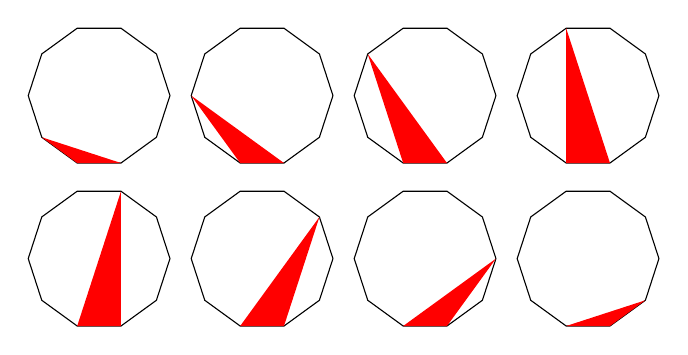
\begin{tikzpicture}
      \def\dr{2}
      \def\spc{2.3*\dr}

      \decagon{0*\spc}{\spc}{\dr}{-\dec@aii}{-\dec@bi}
      \decagon{1*\spc}{\spc}{\dr}{-1}{0}
      \decagon{2*\spc}{\spc}{\dr}{-\dec@aii}{\dec@bi}
      \decagon{3*\spc}{\spc}{\dr}{-\dec@ai}{\dec@bii}

      \decagon{0*\spc}{0}{\dr}{\dec@ai}{\dec@bii}
      \decagon{1*\spc}{0}{\dr}{\dec@aii}{\dec@bi}
      \decagon{2*\spc}{0}{\dr}{1}{0}
      \decagon{3*\spc}{0}{\dr}{\dec@aii}{-\dec@bi}
    \end{tikzpicture}
  \end{center}

  The area of each decagon is $240$.
  What is the total area of all the red triangles?
}

\def\advent@xxi@viii{
  The sum of three integers is $51$.
  The product of the same three integers is $836$. What is the product of largest integer and the second-largest integer?
}

\def\advent@xxi@ix{
  Eve writes down a sequence of consecutive positive integers (she writes more than one number).
  The sum of the numbers Eve has written down is $844$.
  Today's number is the smallest integer that Eve has written down.
}

\def\advent@xxi@x{
  Put the digits $1$ to $9$ (using each digit exactly once) in the boxes so that the sums are correct.
  Today's number is the largest number you can make using the digits in the red boxes.

  \grid@advent@xxi@x{}{}{}{}{}{}{}{}{}
}

\def\advent@xxi@xi{
  The integers are written in a triangle as shown below:
  \begin{center}
    \begin{tabular}{ccccccc}
         &    &    & 1    &    &    &    \\
         &    & 2  & 3    & 4  &    &    \\
         & 5  & 6  & 7    & 8  & 9  &    \\
      10 & 11 & 12 & 13   & 14 & 15 & 16 \\
         &    &    & etc. &    &    &
    \end{tabular}
  \end{center}
  Today's number appears directly above the number $750$ in the triangle of integers.
}

\def\advent@xxi@abgrid{
  \begin{center}
    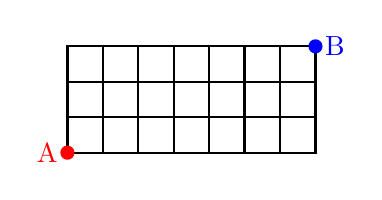
\begin{tikzpicture}
      \def\gs{1}
      % Grid
      \foreach \i in {0,...,6}{
          \foreach \j in {0,...,2}{
              \draw[thick] (\i * \gs, \j * \gs) rectangle (\i * \gs + \gs, \j * \gs + \gs);
            }
        }
      % Points
      \fill[color=red] (0, 0) circle (0.2) node[color=red,left] {A};
      \fill[color=blue] (7*\gs, 3*\gs) circle (0.2) node[color=blue,right] {B};
    \end{tikzpicture}
  \end{center}
}
\def\advent@xxi@xii{
  You start at the point marked A in the picture below. You want to get to the point marked B.
  You may travel \textbf{to the right} or \textbf{upwards} along the black lines.

  \advent@xxi@abgrid

  Today's number is the total number of possible routes to get from A to B.
}

\def\advent@xxi@xiii{
  The diagram below shows three circles and two triangles.
  The three circles all meet at one point.
  The vertices of the smaller red triangle are at the centers of the circles.
  The lines connecting the vertices of the larger blue triangle to the point where all three circles meet are diameters of the three circles.

  \begin{center}
    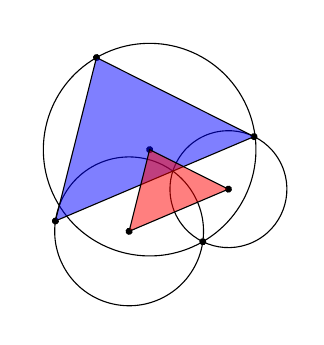
\begin{tikzpicture}[rotate=30,transform shape]
      \def\bcr{3}
      \def\scr{0.55*\bcr}
      \def\sca{34}
      \def\mcr{0.7*\bcr}
      \def\mca{142}
      \def\pr{0.1}

      % Circles
      \draw (0, \bcr) circle (\bcr);
      \draw (\sca: \scr) circle (\scr);
      \draw (\mca: \mcr) circle (\mcr);

      % Points
      \fill (0, 0) circle (\pr);
      \fill (0, \bcr) circle (\pr);
      \fill (0, 2*\bcr) circle (\pr);
      \fill (\sca: \scr) circle (\pr);
      \fill (\sca: 2*\scr) circle (\pr);
      \fill (\mca: \mcr) circle (\pr);
      \fill (\mca: 2*\mcr) circle (\pr);

      % Triangles
      \draw[fill=blue,fill opacity=0.5] (\mca: 2*\mcr) -- (0, 2*\bcr) -- (\sca: 2*\scr) -- cycle;
      \draw[fill=red,fill opacity=0.5] (\mca: \mcr) -- (0, \bcr) -- (\sca: \scr) -- cycle;
    \end{tikzpicture}
  \end{center}

  The area of the smaller red triangle is $226$.
  What is the area of the larger blue triangle?
}

\def\advent@xxi@xiv{
  You start at the point marked A in the picture below.
  You want to get to the point marked B.
  You may travel \textbf{to the right}, \textbf{upwards}, or \textbf{to the left} along the black lines, but you cannot pass along the same line segment more than once.

  \advent@xxi@abgrid

  Today's number is the total number of possible routes to get from A to B.
}

\newcommand\pyramid@advent@xxi@xvi[6]{
  \begin{center}
    \begin{tabular}{cccccc}
      (row 1) &    &    & #1   &    &    \\
      (row 2) &    & #2 &      & #3 &    \\
      (row 3) & #4 &    & #5   &    & #6 \\
              &    &    & etc. &    &
    \end{tabular}
  \end{center}
}
\def\advent@xxi@xv{
  The odd numbers are written in a pyramid.

  \pyramid@advent@xxi@xvi{1}{3}{5}{7}{9}{11}

  What is the mean of the numbers in the 19th row?
}

\newcommand\grid@advent@xxi@xvi[9]{
  \begin{center}
    \begin{tikzpicture}[scale=2]
      \gridbox{0}{2}{#1}
      \gridbox{1}{2}{#2}
      \gridbox{2}{2}{#3}
      \gridbox{0}{1}{#4}
      \gridbox{1}{1}{#5}
      \gridbox{2}{1}{#6}
      \gridbox{0}{0}{#7}
      \gridbox{1}{0}{#8}
      \gridbox{2}{0}{#9}

      % Labels
      \cwlab{0}{2}{1}
      \cwlab{1}{2}{2}
      \cwlab{2}{2}{3}
      \cwlab{0}{1}{4}
      \cwlab{0}{0}{5}
    \end{tikzpicture}
  \end{center}
}
\def\advent@xxi@xvi{
  Each clue in this crossnumber is formed of two parts connected by a logical connective: AND means that both parts are true; NAND means that at most one part is true; OR means that at least one part is true; NOR means that neither part is true; XOR means that exactly one part is true; XNOR means that either both parts are false or both parts are true.
  No number starts with $0$.

  \begin{multicols}{2}
    \grid@advent@xxi@xvi{}{}{}{}{}{}{}{}{}

    \columnbreak

    \begin{enumerate}
      \item \textbf{1A} is a palindrome XNOR \textbf{1D} is a palindrome.
      \item \textbf{1A} is greater than $350$ NOR \textbf{1D} is less than $150$.
      \item \textbf{3D} is odd NAND \textbf{4A} and \textbf{2D} are equal.
      \item \textbf{3D} is prime XOR \textbf{5A} is odd.
      \item \textbf{4A} is a cube AND \textbf{2D} is a cube.
      \item The sum of the digits of \textbf{3D} is $2$ OR the sum of the digits of \textbf{5A} is $5$.
      \item Today's number is \textbf{1D}.
    \end{enumerate}
  \end{multicols}
}

\def\advent@xxi@xvii{
  The digital product of a number is computed by multiplying together all of its digits. For example, the digital product of $6273$ is $252$.

  Today's number is the smallest number whose digital product is $252$.
}

\def\advent@xxi@xviii{
  Put the digits $1$ to $9$ (using each digit exactly once) in the boxes so that the sums are correct.
  The sums should be read left to right and top to bottom ignoring the usual order of operations.
  For example, $4 + 3 \times 2$ is $14$, not $10$.
  Today's number is the product of the numbers in the red boxes.

  \grid@advent@xxi@xviii{}{}{}{}{}{}{}{}{}
}

\def\advent@xxi@xix{
  The equation $352x^3 - 528x^2 + 90 = 0$ has three distinct real-valued solutions.

  Today's number is the number of integers $a$ such that the equation $352x^3 - 528x^2 + a = 0$ has three distinct real-valued solutions.
}

\def\advent@xxi@xx{
  What is the area of the largest area triangle that has one side of length $32$ and one side of length $19$?
}

\newcommand\grid@advent@xxi@xxi[9]{
  \begin{center}
    \begin{tikzpicture}
      \bigbox{0}{3}{#1}
      \bigbox{1}{3}{#2}
      \bigbox{2}{3}{#3}
      \bbtextr{3}{3}{\textbf{today's number}}

      \bigbox{0}{2}{#4}
      \bigbox{1}{2}{#5}
      \bigbox{2}{2}{#6}
      \bbtextr{3}{2}{prime}

      \bigbox{0}{1}{#7}
      \bigbox{1}{1}{#8}
      \bigbox{2}{1}{#9}
      \bbtextr{3}{1}{square}

      \bbtextb{0}{0}{cube}
      \bbtextb{1}{0}{odd}
      \bbtextb{2}{0}{multiple\\of $11$}
    \end{tikzpicture}
  \end{center}
}
\def\advent@xxi@xxi{
  Arrange the digits $1$–$9$ (using each digit exactly once) so that the three digit number in: the middle row is a prime number; the bottom row is a square number; the left column is a cube number; the middle column is an odd number; the right column is a multiple of $11$.
  The $3$-digit number in the first row is today's number.

  \grid@advent@xxi@xxi{}{}{}{}{}{}{}{}{}
}

\def\advent@xxi@xxii{
  There are $12$ ways of placing $2$ tokens on a $2 \times 4$ grid so that no two tokens are next to each other horizontally, vertically or diagonally:

  \begin{center}
    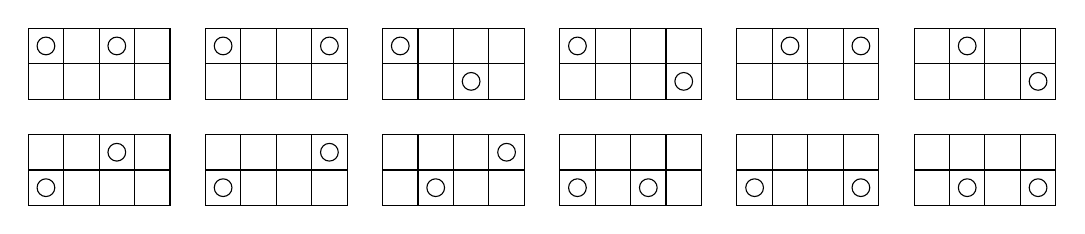
\begin{tikzpicture}
      % Draw all the grids
      \foreach \gi in {0,1}{
          \foreach \gj in {0,...,5}{
              \foreach \i in {0,1}{
                  \foreach \j in {0,...,3}{
                      \gridbox{5*\gj + \j}{3*\gi + \i}{}
                    }
                }
            }
        }

      % Place token circles
      \gridcirc{0}{4}
      \gridcirc{2}{4}
      \gridcirc{5}{4}
      \gridcirc{8}{4}
      \gridcirc{10}{4}
      \gridcirc{12}{3}
      \gridcirc{15}{4}
      \gridcirc{18}{3}
      \gridcirc{21}{4}
      \gridcirc{23}{4}
      \gridcirc{26}{4}
      \gridcirc{28}{3}
      \gridcirc{0}{0}
      \gridcirc{2}{1}
      \gridcirc{5}{0}
      \gridcirc{8}{1}
      \gridcirc{11}{0}
      \gridcirc{13}{1}
      \gridcirc{15}{0}
      \gridcirc{17}{0}
      \gridcirc{20}{0}
      \gridcirc{23}{0}
      \gridcirc{26}{0}
      \gridcirc{28}{0}
    \end{tikzpicture}
  \end{center}

  Today's number is the number of ways of placing $2$ tokens on a $2 \times 21$ grid so that no two tokens are next to each other horizontally, vertically or diagonally.
}

\def\advent@xxi@xxiii{
  I draw the parabola $y = x^2$ and mark points on the parabola at $x = 17$ and $x = -6$.
  I then draw a straight line connecting these two points.

  At which value of $y$ does this line intercept the $y$-axis?
}

\def\advent@xxi@xxiv{
  The digital product of a number is computed by multiplying together all of its digits.
  For example, the digital product of $1522$ is $20$.

  How many $12$-digit numbers are there whose digital product is $20$?
}

\def\card@xxi@i{
  What is the sum of all the odd integers between $0$ and $30$?
}

\def\card@xxi@ii{
  What is the sum of all the odd integers between $0$ and $5668$?
}

\def\card@xxi@iii{
  What is the smallest integer with a digital sum of $28$ and a digital product of $10000$?
}

\def\card@xxi@iv{
  What is the smallest integer with a digital sum of $41$ and a digital product of $432000$?
}

\def\card@xxi@v{
  What is the area of the largest area dodecagon that will fit inside a circle with area $111185 \pi$?
}

\def\card@xxi@vi{
  What is the area of the largest area heptagon that will fit inside a semicircle with area $115185 \pi$?
}

\def\card@xxi@vii{
  How many terms are there in the (simplified) expansion of $(x + y + z)^2$?
}

\def\card@xxi@viii{
  How many terms are there in the (simplified) expansion of $(x + y + z)^{41172}$?
}

\def\card@xxi@ix{
  What is the largest integer that cannot be written as $4a + 5b$ for non-negative integers $a$ and $b$?
}

\def\card@xxi@x{
  What is the largest integer that cannot be written as $83409a + 66608b$ for non-negative integers $a$ and $b$?
}

\def\card@xxi@xi{
  How many positive integers are there below $100$ whose digits are all non-zero and different?
}

\def\card@xxi@xii{
  How many positive integers are there whose digits are all non-zero and different?
}

\def\card@xxi@xiii{
  What is the only integer for which taking the geometric mean of all its factors (including $1$ and the number itself) gives $2$?
}

\def\card@xxi@xiv{
  What is the only integer for which taking the geometric mean of all its factors (including $1$ and the number itself) gives $25$?
}

\input{boxes}

\begin{document}

\title{MS Scroggs Advent Calendar 2023 Answers}
\author{Dan Whitman}
\date{}

\maketitle

Magic Link: \href{http://mscroggs.co.uk/adventcode/yglswiTw}{http://mscroggs.co.uk/adventcode/yglswiTw}

\aproblem{1}{180}{\advent@xxiii@i}{
  A regular $n$-gon has interior angles that are each
  \gath{
    \theta = \frac{180(n - 2)}{n}
  }
  in degrees.
  Using basic algebra, solving this for $n$ results in
  \gath{
    n = \frac{360}{180 - \theta}
  }
  Therefore, plugging in $\theta = 178$ gives our answer $n = 180$.
}

\aproblem{2}{681}{\advent@xxiii@ii}{
  Clearly, the sum of the first $n$ even numbers and half of the next even number is
  \ali{
    s_n &= \sum_{i=1}^n 2i + \frac{2(n+1)}{2} = 2 \sum_{i=1}^n i + (n+1) = 2\frac{n(n+1)}{2} + (n+1) \non
    &= n(n+1) = (n+1) = (n+1)^2.
  }
  Solving this for $n$ clearly results in
  \gath{
    n = \sqrt{s_n} - 1.
  }
  Hence, the $n$ we seek is $n = \sqrt{465124} - 1 = 682 - 1 = 681$.
  This answer was verified with a Python program that calculates the actual sum $s_{681}$, showing that this is indeed $465124$.
}

\aproblem{3}{195}{\advent@xxiii@iii}{
  Let $n$ be this smallest multiple of $15$ whose digits add up to $15$.
  First, we note that clearly the digits of $555$ add to $15$, and that $555 = 37 \times 15$, and so is also a multiple of $15$.
  Therefore, it has to be that $n \leq 555$.

  Now, any multiple of $15$ must end in either the digits $0$ or $5$.
  Suppose that the last digit is $0$ so that $n$ has the form $n = d_2 d_10$, and thus $d_2 + d_1 = 15$.
  There are only two sets of digits such that this is the case, namely $6 + 9 = 9 + 6 = 15$ and $7 + 8 = 8 + 7 = 15$.
  This is because $d_2 \leq 5$ would require that $d_1 > 9$ and vice versa.
  Therefore, it has to be that $d_2 \in \braces{6, 7, 8, 9}$, which would mean that $n = d_2 d_1 0 > 555$.
  Hence, it must be that the last digit is a $5$.

  Thus, $n$ has the form $n = d_2 d_1 5$.
  If it were the case that $d_2 = 0$ so that $n$ was a two-digit number, it would have to be that $0 + d_1 + 5 = 15$ so that $d_1 = 10$, which is clearly out of the range of valid digits.
  Therefore, $0 < d_2 \leq 5$.
  What about if $d_2 = 1$?
  Well, in this case, we'd have $1 + d_2 + 5 = 15$ so that $d_2 = 9$.
  Hence, the digits of $n = 195$ sum to $15$.
  Since also $195 = 13 \times 15$, this is in fact our answer since there can be no smaller number that meets the established criteria!

  This answer was also verified using a brute force Python program.
}

\aproblem{4}{246}{\advent@xxiii@iv}{
  Let us generalize this a bit and ask, for any positive integer $a$, what is the largest value of $n$ for which $f(n) = (n! - a)/(n - a)$ is an integer?

  First, for $n = 2a$ we have
  \gath{
    f(n) = f(2a) = \frac{(2a)! - a}{2a - a} = \frac{2a(2a-1)! - a}{a} = 2(2a-1)! - 1,
  }
  which is clearly an integer. We aim to prove that, in fact, $n = 2a$ is the \emph{largest} $n$ for which $f(n)$ is an integer!

  To this end, first note that $f(n)$ being an integer means that $n! - a$ is divisible by $n - a$, which is equivalent to saying that
  \gath{
    n! - a \equiv 0 \pmod{n-a}. \label{eqn:04:fcond}
  }
  Now suppose that $n > 2a$ so that
  \gath{
    a > 0 \non
    n > 2a > a \non
    n - a > a > 0.
  }
  We also clearly have
  \gath{
    n > n - a
  }
  since $a > 0$.
  Therefore, clearly
  \gath{
    n! = (n-a)k,
  }
  where $k$ is an integer.
  Hence, $n!$ is a multiple of $n-a$ so that
  \gath{
    n! \equiv 0 \pmod{n-a}.
  }
  From this it follows that
  \gath{
    n! - a \equiv -a \pmod{n-a},
  }
  and, since $0 < a < n-a$, this means that \eqref{eqn:04:fcond} cannot be true so that $f(n)$ cannot be an integer!

  In our case, we have $a = 123$ so that our answer is $n = 2 \cdot 123 = 246$.
  This answer was also verified using a brute force Python program.
}

\aproblem{5}{378}{\advent@xxiii@v}{
  \boxans{\gridsol@advent@xxiii@v}
}

\newcommand\table@vi[1]{
  \begin{center}
    \begin{tabular}{c|c}
      $n$ & $N_n$ \\
      \hline
      #1
    \end{tabular}
  \end{center}
}
\aproblem{6}{233}{\advent@xxiii@vi}{
  Consider the general problem of the number of ways to tile an $n \times 2$ rectangle with $2 \times 1$ pieces, and let this number be $N_n$.
  Clearly the number of ways to tile a $1 \times 2$ rectangle is just one, and hence $N_1 = 1$.
  Similarly, there are obviously only two ways to tile a $2 \times 2$ square, namely the following:
  \begin{center}
    \begin{tikzpicture}[scale=\crscale]
      \crvert{cry}{0}{0}
      \crvert{crb}{1}{0}

      \crhorz{cry}{3}{0}
      \crhorz{crb}{3}{-1}
    \end{tikzpicture}
  \end{center}
  Therefore, of course, $N_2 = 2$.

  Now, if we consider $N_n$, we have two cases, either the first $2 \times 1$ tile is oriented vertically or horizontally.
  In the first case, the width of the first tile is only~1 so that the remaining part is an $(n-1) \times 2$ rectangle as shown below:
  \begin{center}
    \begin{tikzpicture}[scale=\crscale]
      \crvert{cry}{0}{0}
      \filldraw[ultra thick,fill=crg] (1,0) rectangle (10,-2);
      \node at (6, -1) {$(n-1) \times 2$};
    \end{tikzpicture}
  \end{center}
  Therefore, the number of tilings in this case is simply $N_{n-1}$.
  In the second case in which the first tile is horizontal, the second tile must also be horizontal beneath, and their width is~2 so that the remaining part is an $(n-2) \times 2$ rectangle.
  This is illustrated below:
  \begin{center}
    \begin{tikzpicture}[scale=\crscale]
      \crhorz{cry}{0}{0}
      \crhorz{crb}{0}{-1}
      \filldraw[ultra thick,fill=crg] (2,0) rectangle (10,-2);
      \node at (6, -1) {$(n-2) \times 2$};
    \end{tikzpicture}
  \end{center}
  Thus, the total number of tilings in this case is $N_{n-2}$.
  As these cases are exhaustive, the total number of tilings is
  \gath{
    N_n = N_{k-1} + N_{k-2},
  }
  but this is just a Fibonacci sequence!
  Putting this all together we clearly have
  \begin{multicols}{3}
    \table@vi{
      1   & 1     \\
      2   & 2     \\
      3   & 3     \\
      4   & 5     \\
    }
    \columnbreak
    \table@vi{
      5   & 8     \\
      6   & 13    \\
      7   & 21    \\
      8   & 34    \\
    }
    \columnbreak
    \table@vi{
      9   & 55    \\
      10  & 89    \\
      11  & 144   \\
      12  & 233   \\
    }
  \end{multicols}
  so that our answer is $N_{12} = 233$, which was verified by implementing this sequence in Python.
}

\newcommand\table@vii[1]{
  \begin{center}
    \begin{tabular}{c|c}
      $n$ & $\abs{C_n}$ \\
      \hline
      #1
    \end{tabular}
  \end{center}
}
\aproblem{7}{987}{\advent@xxiii@vii}{
  For $n \geq 0$, let $I_n$ be the set containing the numbers $1$ to $n$ inclusive, that is
  \gath{
    I_n = \braces{k \in \ints \mid 1 \leq k \leq n}.
  }
  Similarly, let $C_n$ be the set of subsets of $I_n$ that do not include any consecutive numbers, including the empty set.
  Clearly, we have that $I_0 = \es$, and so $C_0 = \braces{\es}$ and $\abs{C_0} = 1$.
  We also have that $I_1 = \braces{1}$ so that
  \gath{
    C_1 = \braces{\varnothing, \braces{1}},
  }
  and hence $\abs{C_1} = 2$.
  Now consider any $n > 1$ so that $I_n = \braces{1, 2, \ldots, n-1, n}$.
  For any set in $C_n$, either $n$ is in the set or it is not.
  Consider those sets of $C_n$ such that $n$ is \emph{not} in any of the sets.
  The set of these is clearly simply $C_{n-1}$.
  Now consider the sets of $C_n$ where $n$ is in all the sets.
  This means that $n-1$ cannot be in any of the sets since it is consecutive with $n$.
  Thus, these are exactly the sets $\braces{S \cup \braces{n} \mid S \in C_{n-2}}$, which of course has the same cardinality as $C_{n-2}$.
  Since the cases are exhaustive and the set of subsets in each case are clearly disjoint (since none of the sets of one contain $n$ while all the sets of the other contain $n$), it follows that
  \gath{
    \abs{C_n} = \abs{C_{n-1}} + \abs{C_{n-2}}
  }
  so that the sequence $\abs{C_n}$ is a Fibonacci sequence!
  It is then easy to calculate this sequence:
  \begin{multicols}{3}
    \table@vii{
      0   & 1           \\
      1   & 2           \\
      2   & 3           \\
      3   & 5           \\
      4   & 8           \\
    }
    \columnbreak
    \table@vii{
      5   & 13          \\
      6   & 21          \\
      7   & 34          \\
      8   & 55          \\
      9   & 89          \\
    }
    \columnbreak
    \table@vii{
      10  & 144         \\
      11  & 233         \\
      12  & 377         \\
      13  & 610         \\
      14  & 987         \\
    }
  \end{multicols}
  Note hat $\abs{C_4} = 8$ as expected from the example.
  Our answer is then $\abs{C_{14}} = 987$, which was verified using a brute force Python program that filters the power sets of $I_n$ to only those subsets containing non-consecutive integer.
}

\aproblem{8}{729}{\advent@xxiii@viii}{
  Suppose that $n$ is a positive, odd integer so that $n = 2k+1$ for some integer $k \geq 0$.
  Also suppose that we write the inverted triangle of numbers as above where the first row is from $1$ to $n$.
  Since $n$ is odd, there is a number $m$ exactly in the middle of the first row with the property that there are exactly $m-1$ numbers to the left of it (i.e. $1$ through $m-1$) and $m-1$ to the right (i.e. $m+1$ through $n$).
  So the numbers of numbers on the right is
  \gath{
    m - 1 = n - m \non
    2m = n + 1 \non
    2m = (2k + 1) + 1 \non
    2m = 2(k+1) \non
    m = k+1
  }
  so that we have our middle number.
  It should then be clear that there are $m$ rows, and let us number them from $1$ to $m$ from top to bottom, noting that row $r$ starts with the number $r$ and ends with $n - r + 1$.
  The last row then contains only $m = k+1$, noting that the last number is also $n - m + 1 = (2k+1) - (k+1) + 1 = k + 1 = m$.

  A short digression before we proceed: for non-negative integers $a \leq b$, we have that
  \gath{
    \sum_{i=a}^b i = \sum_{i=1}^b i - \sum_{i=1}^{a-1} i = \frac{b(b+1)}{2} - \frac{(a-1)a}{2} = \frac{b(b+1) - a(a-1)}{2}.
  }
  This still holds if $a = 0$ if we adopt the usual convention that $\sum_{i=a}^b f(i) = 0$ whenever $b < a$.
  So we then have that the sum of the numbers in row $r$ is
  \ali{
    S_r &= \sum_{i=r}^{n-r+1} i = \sum_{i=r}^{(2k+1)-r+1} i = \sum_{i=r}^{2(k+1)-r} i = \sum_{i=r}^{2m-r} i = \frac{(2m - r)(2m - r + 1) - r(r-1)}{2} \non
    &= \frac{4m^2 - 2m r + 2m - 2m r + r^2 - r - r^2 + r}{2} = \frac{4m^2 - 4m r + 2m}{2} = \frac{2m(2m - 2r + 1)}{2} \non
    &= m(2m - 2r + 1)
  }
  The total sum of all rows is then
  \ali{
    S &= \sum_{r=1}^m S_r = \sum_{r=1}^m m(2m - 2r + 1) = m\squares{\sum_{r=1}^m(2m + 1) - 2\sum_{r=1}^m r} \non
    &= m \squares{m(2m + 1)- 2\frac{m(m+1)}{2}} = m^2 \squares{2m + 1 - (m+1)} = m^3 \non
    &= (k+1)^3.
  }
  In our case, we have that $n = 17 = 2 \cdot 8 + 1$ so that $k = 8$.
  Thus, the sum we seek is $S = (k+1)^3  = 9^3 = 729$.
  This answer was verified with a brute force Python program that calculates the sum directly.
}

\aproblem{9}{600}{\advent@xxiii@ix}{
  Consider the more general case when the length of the red lines is $a$, which is also the length of the blue lines.
  Let $w$ and $h$ denote the width and height of the rectangle, respectively.
  Then the sum of the blue lines is of course
  \gath{
    w + h = a. \label{eqn:09:add}
  }
  One corner of the rectangle along with one of the red lines forms a right triangle with sides $w/2$ and $h$, and a hypotenuse of $a/2$.
  Thus, we have
  \gath{
    \parens{\frac{w}{2}}^2 + h^2 = \parens{\frac{a}{2}}^2 \non
    \frac{w^2}{4} + h^2 = \frac{a^2}{4} \non
    w^2 + 4h^2 + a^2. \label{eqn:09:tri}
  }
  From \eqref{eqn:09:add} we have $w = a - h$, so substituting this into \eqref{eqn:09:tri} gives us
  \gath{
    (a - h)^2 + 4h^2 = a^2 \non
    a^2 - 2ah + h^2 + 4h^2 = a^2 \non
    5h^2 - 2ah = 0 \non
    5h^2 = 2ah \non
    h = \frac{2a}{5}
  }
  Substituting this back into \eqref{eqn:09:add} yields
  \gath{
    w + \frac{2a}{5} = a \non
    w = a\parens{1 - \frac{2}{5}} \non
    w = \frac{3a}{5}.
  }
  Hence, the area is
  \gath{
    A = wh = \parens{\frac{3a}{5}}\parens{\frac{2a}{5}} = \frac{6a^2}{25}.
  }
  In our case, we have $a = 50\unit{cm}$, and therefore our answer is $A = 6 \cdot 50^2/25 = 600\unit{cm^2}$.
}

\aproblem{10}{450}{\advent@xxiii@x}{
  Let $E$ be any even number and $O$ be any odd number.
  It is trivial to show that
  \gath{
    E + E = E \\
    E + O = O + E = O \\
    O + O = E.
  }
  Now note that clearly the sum of the digits of $1000$ is one and so odd, so we need only consider three-digit numbers where the first digit is nonzero.
  There are $5$ even digits (i.e. $\braces{0, 2, 4, 6, 8})$ and $5$ odd digits (i.e. $\braces{1,3,5,7,9}$).
  However, the first digit must be nonzero, so that there are only $4$ possible even number that can be in this position.

  We consider all combinations of whether each digit is even or odd, and denote the parity of each position.
  For example a parity signature of $EOE$ would denote a number where the first digit is even, the second odd, and the third even.
  Note that two sets of numbers with different parity signatures are disjoint since the sets of even and odd digits are disjoint.
  For signatures whose digits sum to an even number, we also calculate the number of such numbers by considering the number of possibilities of each digit given the caveat about the first digit when even.
  Hence, given the addition rules above, we have
  \begin{center}
    \begin{tabular}{ccc}
      Signature & Digital sum & Number of numbers         \\
      \hline
      $EEE$     & $E$         & $4 \cdot 5 \cdot 5 = 100$ \\
      $EEO$     & $O$         &                           \\
      $EOE$     & $O$         &                           \\
      $EOO$     & $E$         & $4 \cdot 5 \cdot 5 = 100$ \\
      $OEE$     & $O$         &                           \\
      $OEO$     & $E$         & $5 \cdot 5 \cdot 5 = 125$ \\
      $OOE$     & $E$         & $5 \cdot 5 \cdot 5 = 125$ \\
      $OOO$     & $O$         &                           \\
    \end{tabular}
  \end{center}
  Therefore, the total number of numbers with even digital sums is the sum of the numbers in the final column: $100 + 100 + 125 + 125 = 450$.
  This result was verified with a brute force Python program.
}

\aproblem{11}{TODO}{\advent@xxiii@xi}{
  \boxans{\gridsol@advent@xxiii@xi}
}

\aproblem{12}{TODO}{\advent@xxiii@xii}{
  TODO
}

\aproblem{13}{TODO}{\advent@xxiii@xiii}{
  TODO
}

\end{document}
